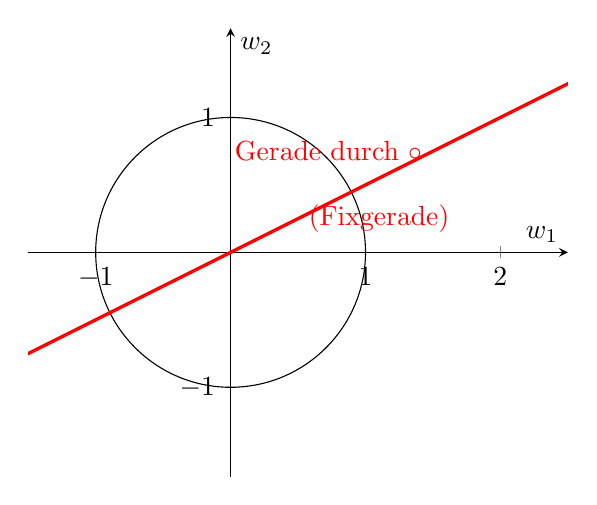
\begin{tikzpicture}
	\begin{axis}[
		axis lines=middle,
		axis equal,
		xmin=-1.5,
		xmax=2.5,
		ymin=-1,
		ymax=1,
		xlabel=$w_1$,
		ylabel=$w_2$,
		]	
		\draw (axis cs: 0, 0) circle [radius=1];
		\addplot[-, red, very thick] {0.5*x} node[above, left, red, pos=0.65] {Gerade durch $\circ$} node[below, right, red, pos=0.55] {(Fixgerade)};
	\end{axis}
\end{tikzpicture}